\addcontentsline{toc}{chapter}{Занятие 8. Стационарные случайные процессы}
\chapter*{Занятие 8. Стационарные случайные процессы}

\addcontentsline{toc}{section}{Контрольные вопросы и задания}
\section*{Контрольные вопросы и задания}

\subsubsection*{Приведите определение случайного процесса, стационарного в широком смысле.}

$ \xi \left( t \right), \, t \in T$ называется стационарным в широком смысле (стационарным), если
\begin{enumerate}
  \item $m \left( t \right) \equiv m \, \left( const \right) $;
  \item $K \left( t, s \right) = K \left( t + r, s + r \right), \, \forall t, s, r \in T$.
  Это означает, что ковариационная функция --- это сейчас функция разности аргументов,
  то есть $K \left( t, s \right) = k \left( t - s \right) $.
\end{enumerate}

\subsubsection*{Приведите определение ковариационной функции случайного процесса.}

$K \left( t, s \right) =
  M \left[ \xi \left( t \right) - m \left( t \right) \right] \cdot
  \left[ \xi \left( s \right) - m \left( s \right) \right], \,
  t, s \in T$.

\subsubsection*{Сформулируйте теорему Бохнера про спектральное изображения ковариационной функции
                стационарного в широком смысле случайного процесса.}

Пусть $ \xi \left( t \right), \, t \in \mathbb{R}$ ---
это стационарный и непрерывный в среднем квадратическом случайный процесс.
Тогда существует конечная мера $ \mu $ на $ \mathbb{R}$ такая, что
$$k \left( t \right) =
  \int \limits_{-\infty}^{+\infty} e^{it \lambda } \mu \left( d \lambda \right),$$
мера $ \mu $ определяется единственным образом.

\subsubsection*{Что называется спектральной функцией, спектральной плотностью стационарного в
                широком смысле случайного процесса?}

$ \mu $ называеься спектральной мерой, а если есть плотность $p$, то $p$ ---
это спектральная плотность.

\addcontentsline{toc}{section}{Аудиторные задачи}
\section*{Аудиторные задачи}

\subsubsection*{8.2}

\textit{Задание.}
Пусть $A, \eta, \varphi $ --- независимые случайные величины,
причём $ \varphi $ имеет равномерное распределение на отрезке $ \left[ 0, 2 \pi \right] $.
Докажите, что процесс
$ \left\{
    \xi \left( t \right) = A \cos \left( t \eta + \varphi \right), \, t \in \mathbb{R}
  \right\} $
является стационарным в широком смысле.

\textit{Решение.}
$$M \xi \left( t \right) =
  M \left[ A \cos \left( \eta t + \varphi \right) \right] =
  MA \cdot M \cos \left( \eta t + \varphi \right) =$$
Распишем косинус суммы
$$= MA \cdot M \left[
    \cos \left( \eta t \right) \cos \varphi - \sin \left( \eta t \right) \sin \varphi \right] =$$
Все множители независимы
$$= MA \cdot M \cos \left( \eta t \right) \cdot M \cos \varphi -
  MA \cdot M \sin \left( \eta t \right) \cdot M \sin \varphi =$$
Сгруппируем множители
$$= M \left[ A \cos \left( \eta t \right) \right] \cdot M \cos \varphi -
  M \left[ A \sin \left( \eta t \right) \right] \cdot M \sin \varphi =$$
Запишем математическое ожидание $ \sin \varphi $
через интеграл от плотности равномерного распределения
$$= M \left[ A \cos \left( \eta t \right) \right]
  \int \limits_{ \mathbb{R}} \cos x \cdot p \left( x \right) dx -
  M \left[ A \sin \left( \eta t \right) \right]
  \int \limits_{ \mathbb{R}} \sin x \cdot p \left( x \right) dx =$$
Подставим плотность
$$= M \left[ A \cos \left( \eta t \right) \right] \int \limits_0^{2 \pi } \cos xdx -
  M \left[ A \sin \left( \eta t \right) \right] \int \limits_0^{2 \pi } \sin xdx =$$
Возьмём интегралы
$$= M \left[ A \cos \left( \eta t \right) \right] \cdot \left. \sin x \right|_0^{2 \pi } -
  M \left[ A \sin \left( \eta t \right) \right] \cdot
  \left. \left( - \cos x \right) \right|_0^{2 \pi } =
  0.$$

Ковариационная функция
$$K \left( t, s \right) =
  M \xi \left( t \right) \xi \left( s \right) =
  M A^2 \cdot M \cos \left( \eta t + \varphi \right) \cdot \cos \left( \eta s + \varphi \right) =$$
Распишем произведение косинусов
$$= \frac{MA^2}{2} \cdot \left\{
  M \cos \left[ \eta \left( t + s \right) + 2 \varphi \right] +
  M \cos \left[ \eta \left( t - s \right) \right] \right\} =$$
Первое слагаемое равно нулю
$$= \frac{MA^2}{2} \cdot M \cos \left[ \eta \left( t - s \right) \right].$$
Значит, процесс стационарный.

\subsubsection*{8.3}

\textit{Задание.}
Пусть $ \left\{ N \left( t \right), \, t \geq 0 \right\} $ ---
процесс Пуассона с параметром $ \lambda $.
Докажите, что процесс
$ \left\{ \xi \left( t \right) = N \left( t + 1 \right) - N \left( t \right), \, t \geq 1 \right\} $
является стационарным в широком смысле.

\textit{Решение.}
$ \left\{ \xi \left( t \right) = N \left( t + 1 \right) - N \left( t \right), \, t \geq 1 \right\} $
--- процесс приращений пуассоновского процесса.

\begin{enumerate}
  \item
  $$M \xi \left( t \right) =
    M \left[ N \left( t + 1 \right) - N \left( t \right) \right] =
    MN \left( t + 1 \right) - MN \left( t \right) =
    \lambda \left( t + 1 \right) - \lambda t =
    \lambda,$$
  то есть математическое ожидание постоянное.
  \item Теперь найдём ковариационную функцию
  $$K \left( t, s \right) =
    cov \left[ \xi \left( t \right), \xi \left( s \right) \right] =
    cov \left[
      N \left( t + 1 \right) - N \left( t \right),
      N \left( s + 1 \right) - N \left( s \right) \right] =$$
  Известно, что
  $cov \left[ N \left( t \right), N \left( s \right) \right] =
    \lambda \min \left( t, s \right) $.
  Раскрываем ковариацию и получаем 4 слагаемых
  $$= \lambda \left[
      \min \left( t + 1, s + 1 \right) - \min \left( t + 1, s \right) -
      \min \left( t, s + 1 \right) + \min \left( t, s \right) \right] =$$
  Возможные случаи изображены на рисунке \ref{fig:83}.

  \begin{figure}[h!]
    \centering
    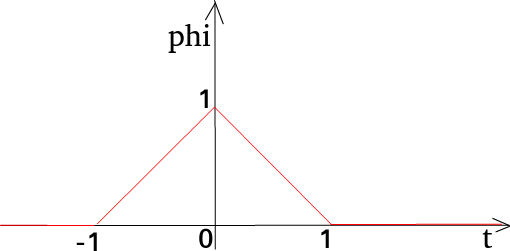
\includegraphics[width=.4\textwidth]{./pictures/4_2.png}
    \caption{Возможные случаи (два последних симметричны двум первым)}
    \label{fig:83}
  \end{figure}

  В первом случае
  $$= 0.$$
  Во втором случае
  $$= \lambda \left[ s + 1 - t \right].$$

  Запишем ковариационную функцию
  $$K \left( t, s \right) =
    \begin{cases}
      0, \qquad s + 1 \leq t \, \left( 1 \leq t - s \right), \\
      \lambda \left[ 1 - \left( t - s \right) \right],
      \qquad s \leq t \leq s + 1 \, \left( 0 \leq t - s \leq 1 \right), \\
      0, \qquad s \geq t + 1 \, \left( t - s \leq 1 \right), \\
      \lambda \left[ 1 - \left( s - t \right) \right],
      \qquad t \leq s \leq t + 1 \, \left( -1 \leq t - s \leq 0 \right).
    \end{cases}$$

  Надо понять, это функция от разности или нет.
  Условия переписываются через разности, тогда ковариация зависит от разности.

  Сейчас
  $$K \left( t, s \right) =
    \begin{cases}
      0, \qquad \left| t - s \right| \geq 1, \\
      \lambda \left( 1 - \left| t - s \right| \right), \qquad \left| t - s \right| \leq 1.
    \end{cases}$$
\end{enumerate}

\subsubsection*{8.4}

\textit{Задание.}
Пусть $ \left\{ W \left( t \right), \, t \geq 0 \right\} $ --- винеровский процесс.
Надите сектральную функцию процесса
$ \left\{
  \xi \left( t \right) = W \left( t + 1 \right) - W \left( t \right), \, t \geq 0 \right\} $.

\textit{Решение.}
Если $ \left\{ \xi_n, \, n \in \mathbb{Z} \right\} $ ---
это стационарная последовательность с $K \left( n, m \right) = k \left( n - m \right) $,
тогда теорема Герглотца говорит,
что функцию $k$ можно представить как преобразование Фурье какой-то меры, то есть
$$k \left( n \right) =
  \frac{1}{2 \pi } \int \limits_{-\pi }^{ \pi } e^{i \lambda n} \mu \left( d \lambda \right).$$

Эта мера называется спектральной мерой.

Это в слуае дискретного времени.
Для непрерывного времени если
$$ \left\{ \xi \left( t \right), \, t \in \mathbb{R} \right\} $$~---~это стационарный процесс,
непрерывный в $L_2$, его ковариационная функция ---
это $K \left( t, s \right) = k \left( t - s \right) $, в этом случае есть теорема Бохнера,
которая говорит, что
$$k \left( t \right) =
  \frac{1}{2 \pi }
  \int \limits_{-\infty }^{+\infty } e^{i \lambda t} \mu \left( d \lambda \right).$$

Если у этой меры есть плотность, то она называется спектральной плотностью.

$$K \left( t, s \right) =
  \begin{cases}
    1 - \left| t - s \right|, \, \left| t - s \right| \leq 1, \\
    0, \qquad \left| t - s \right| \geq 1.
  \end{cases}$$

Это то же самое, что
$$k \left( t \right) =
  \begin{cases}
    1 - \left| t \right|, \qquad \left| t \right| \leq 1, \\
    0, \qquad \left| t \right| \geq 1.
  \end{cases}$$

Теперь нужно подобрать меру, для которой это --- преобразование Фурье.

Сейчас спектральная плотность
$$p \left( \lambda \right) =
  \int \limits_{-\infty }^{+\infty } k \left( t \right) e^{-i \lambda t} dt =
  \int \limits_{-1}^1 \left( 1 - \left| t \right| \right) e^{-i \lambda t} dt =$$
Экспонента расписывается по формуле Эйлера как сумма косинуса и синуса,
умноженного на мнимую единицу.
Интеграл от синуса равен нулю, так как синус --- нечётная функция, $1 - \left| t \right| $ ---
чётная функция, интегрирование происходит по симметричному отрезку
$$= 2 \int \limits_0^1 \left( 1 - t \right) \cos \lambda t dt =$$
Интегрируем по частям, при этом $1 - \left| t \right| = u$, а $ \cos \lambda t = v$.
Тогда
$$= 2 \left. \left( 1 + t \right) \cdot \frac{ \sin \lambda t}{ \lambda } \right|_0^1 +
  \frac{2}{ \lambda } \int \limits_0^1 \sin \lambda t dt =$$
Первое слагаемое равно нулю
$$= \frac{2}{ \lambda^2} \left( 1 - \cos \lambda \right).$$

\addcontentsline{toc}{section}{Домашнее задание}
\section*{Домашнее задание}

\subsubsection*{8.10}

\textit{Задание.}
Докажите, что сумма независимых стационарных в широком смысле процессов является стационарным в
широком смысле процессом.

\textit{Решение.}
Пусть $ \left\{ \xi_i \left( t \right), \, t \in T \right\}, \, i = \overline{1, n}$ ---
независимые стационарные в широком смысле процессы.
Нужно доказать, что процесс
$$ \left\{
  \eta \left( t \right) = \sum \limits_{i = 1}^n \xi_i \left( t \right), \, t \in T \right\} $$
является стационарным в широком смысле.

$$M \eta \left( t \right) =
  M \sum \limits_{i = 1}^n \xi_i \left( t \right) =
  \sum \limits_{i = 1}^n M \xi_i \left( t \right) =
  \sum \limits_{i = 1}^n m_i =
  m =
  const.$$

Ковариационная функция
$$K \left( t, s \right) =
  cov \left[ \eta \left( t \right), \eta \left( s \right) \right] =
  cov \left[
    \sum \limits_{i = 1}^n \xi_i \left( t \right), \sum \limits_{j = 1}^n \xi_j \left( s \right)
  \right] =$$
Вынесем суммы, так как ковариация --- линейная функция
$$= \sum \limits_{i = 1}^n
    \sum \limits_{j = 1}^n cov \left[ \xi_i \left( t \right), \xi_j \left( s \right) \right] =
  \sum \limits_{i = 1}^n cov \left[ \xi_i \left( t \right), \xi_i \left( s \right) \right] =
  \sum \limits_{i = 1}^n K_i \left( t, s \right) =$$
Все $ \xi_i \left( t \right) $ стационарные,
поэтому их ковариационные функции зависят только от разности аргументов
$$= \sum \limits_{i = 1}^n k_i \left( t - s \right) =
  k \left( t - s \right).$$
Значит, процесс стационарный.

\subsubsection*{8.11}

\textit{Задание.}
Пусть $ \xi_1, \xi_2$ --- независимые одинаково распределённые случайные величины,
которые принимают значения $+1$ и $-1$ с вероятностью $1 / 2$.
Докажите, что процесс
$ \left\{
  \xi \left( t \right) = \xi_1 \cos \lambda t + \xi_2 \sin \lambda t, \, t \in \mathbb{R} \right\} $
является стационарным в широком смысле.

\textit{Решение.}
$$M \xi \left( t \right) =
  M \left( \xi_1 \cos \lambda t + \xi_2 \sin \lambda t \right) =
  M \left( \xi_1 \cos \lambda t \right) + M \left( \xi_2 \sin \lambda t \right) =$$
Вынесем константы
$$= \cos \lambda t \cdot M \xi_1 + \sin \lambda t \cdot M \xi_2 =
  \cos \lambda t \cdot \left( 1 \cdot \frac{1}{2} - 1 \cdot \frac{1}{2} \right) +
  \sin \lambda t \cdot \left( 1 \cdot \frac{1}{2} - 1 \cdot \frac{1}{2} \right) =
  0.$$

Ковариационная функция
$$K \left( t, s \right) =
  M \xi \left( t \right) \xi \left( s \right) =
  M \left[
    \left( \xi_1 \cos \lambda t + \xi_2 \sin \lambda t \right)
    \left( \xi_1 \cos \lambda s + \xi_2 \sin \lambda s \right) \right] =$$
Перемножим скобки
\begin{gather*}
  = \cos \lambda t \cdot \cos \lambda s \cdot M \xi_1^2 +
  \cos \lambda t \cdot \sin \lambda s \cdot M \left( \xi_1 \xi_2 \right) +
  \sin \lambda t \cdot \cos \lambda s \cdot M \left( \xi_2 \xi_1 \right) + \\
  + \sin \lambda t \cdot \sin \lambda s \cdot M \xi_2^2 =
  \cos \lambda t \cdot \cos \lambda s + \sin \lambda t \cdot \sin \lambda s =
  \cos \left[ \lambda \left( t - s \right) \right] = \\
  = k \left( t - s \right).
\end{gather*}
Значит, процесс стационарный.

\subsubsection*{8.12}

\textit{Задание.}
Пусть $ \xi_1, \dotsc, \xi_n, \theta_1, \dotsc, \theta_n$ --- независимые случайные величины,
причём $ \theta_1, \dotsc, \theta_n$ имеют равномерное распределение на $ \left[ 0, 2 \pi \right] $.
Докажите, что процесс
$$ \left\{
    \xi \left( t \right) = \sum \limits_{k = 1}^n \xi_k \cos k \left( \theta_k + t \right)
  \right\} $$
является стационарным в широком смысле.

\textit{Решение.}
$$M \xi \left( t \right) =
  M \sum \limits_{k = 1}^n \xi_k \cos k \left( \theta_k + t \right) =$$
Распишем косинус суммы
$$= \sum \limits_{k = 1}^n
    M \xi_k \cdot
    M \left[
      \cos \left( k \theta_k \right) \cos \left( kt \right) -
      \sin \left( k \theta_k \right) \sin \left( kt \right) \right] =$$
Все множители независимы
$$= \sum \limits_{k = 1}^n
  M \xi_k \cdot
  \left[
    \cos \left( kt \right) \cdot M \cos \left( k \theta_k \right) -
    \sin \left( kt \right) \cdot M \sin \left( k \theta_k \right) \right] =$$
Запишем математическое ожидание $ \cos \left( k \theta_k \right) $ и
$ \sin \left( k \theta_k \right) $ через интеграл от плотности равномерного распределения
$$= \sum \limits_{k = 1}^n
  M \xi_k \left[
    \cos \left( kt \right) \int \limits_{ \mathbb{R}} \cos \left( kx \right) p \left( x \right) dx -
    \sin \left( kt \right) \int \limits_{ \mathbb{R}} \sin \left( kx \right) p \left( x \right) dx
  \right] =$$
Подставим плотность
$$= \sum \limits_{k = 1}^n
  M \xi_k \left[
    \cos \left( kt \right) \int \limits_0^{2 \pi } \cos \left( kx \right) dx -
    \sin \left( kt \right) \int \limits_0^{2 \pi } \sin \left( kx \right) dx \right] =$$
Замена
$$kx = u, \,
  du = kdx, \,
  dx = \frac{du}{k}, \,
  x = 0 \Rightarrow u = 0, \,
  x = 2 \pi \Rightarrow u = 2k \pi.$$
Используя данную замену, получим
$$= \sum \limits_{k = 1}^n
    \frac{M \xi_k}{k} \left[
      \cos \left( kt \right) \int \limits_0^{2k \pi } \cos udu -
      \sin \left( kt \right) \int \limits_0^{2k \pi } \sin udu \right] =$$
Возьмём интегралы
$$= \sum \limits_{k = 1}^n
    \frac{M \xi_k}{k} \left[
      \cos \left( kt \right) \left. \sin u \right|_0^{2k \pi } +
      \sin \left( kt \right) \left. \cos u \right|_0^{2k \pi } \right] =$$
Подставим пределы интегрирования
$$= \sum \limits_{k = 1}^n
    \frac{M \xi_k}{k}
    \left\{
      \cos \left( kt \right) \cdot \sin \left( 2k \pi \right) +
      \sin \left( kt \right) \cdot \left[ \cos \left( 2k \pi \right) - 1 \right] \right\} =$$
Синус в точках 0 и $2 \pi $ равен нулю, а косинус в нуле равен единице
$$= \sum \limits_{k = 1}^n
    \frac{M \xi_k}{k} \left[ 0 + \sin \left( kt \right) \left( 1 - 1 \right) \right] =
  0.$$

Ковариационная функция
$$K \left( t, s \right) =
  cov \left[ \xi \left( t \right), \xi \left( s \right) \right] =
  cov \left[
    \sum \limits_{k = 1}^n \xi_k \cos k \left( \theta_k + t \right),
    \sum \limits_{j = 1}^n \xi_j \cos j \left( \theta_j + s \right) \right] =$$
Вынесем суммы и константы из-под знака ковариации
$$= \sum \limits_{k = 1}^n
    \sum \limits_{j = 1}^n
      \cos k \left( \theta_k + t \right) \cdot
      \cos j \left( \theta_j + s \right) \cdot cov \left( \xi_k, \xi_j \right) =$$
Случайные величины независимы, поэтому ковариация не равна нулю, только если индексы совпадают
$$= \sum \limits_{k = 1}^n
    \cos k \left( \theta_k + t \right) \cdot \cos k \left( \theta_k + s \right) \cdot
    cov \left( \xi_k, \xi_k \right) =$$
Распишем произведение косинусов через сумму
\begin{gather*}
  = \sum \limits_{k = 1}^n
    M \xi_k^2 \cdot \frac{1}{2} \cdot
    \left\{
      \cos \left[ k \left( \theta_k + t - \theta_k - s \right) \right] +
      \cos \left[ k \left( 2 \theta_k + t + s \right) \right] \right\} = \\
  = \frac{1}{2} \sum \limits_{k = 1}^n M \xi_k^2 \cdot \cos \left[ k \left( t - s \right) \right] =
  k \left( t - s \right).
\end{gather*}

Значит, процесс стационарный.

\subsubsection*{8.13}

\textit{Задание.}
Пусть $ \xi \left( t \right) = e^t W \left( e^{-2t} \right), \, t \in \mathbb{R}$,
где $ \left\{ W \left( t \right), \, t \geq 0 \right\} $ --- винеровский процесс.
Докажите, что процесс $ \xi $ является стационарным в широком смысле.
Найдите ковариационную и спектральную функции этого процесса.

\textit{Решение.}
Вычислим математическое ожидание и ковариационную функцию случайного процесса $ \xi $.
Поскольку $W \left( t \right) $ --- винеровский процесс, то
$M \xi \left( t \right) =
  M \left[ e^t W \left( e^{-2t} \right) \right] =
  e^t MW \left( e^{-2t} \right) =
  0$.

Обозначим $ \xi_1 = \xi \left( t_1 \right), \, \xi_2 = \xi \left( t_2 \right), \, t_1 < t_2$.
Тогда
$$K \left( t_1, t_2 \right) =
  M \xi_1 \xi_2 =
  M \left[ e^{t_1} W \left( e^{-2t_1} \right) e^{t_2} W \left( e^{-2t_2} \right) \right] =$$
Вынесем экспоненты
$$= e^{t_1 + t_2} M \left[ W \left( e^{-2t_1} \right) W \left( e^{-2t_2} \right) \right] =
  e^{t_1 + t_2} \min \left( e^{-2t_1}, e^{-2t_2} \right) =
  e^{t_1 + t_2} e^{-2t_2} =$$
Запишем в виде одной экспоненты
$$= e^{t_1 + t_2 - 2t_2} =
  e^{t_1 - t_2}.$$

Таким образом, $K \left( t_1, t_2 \right) = e^{-\left| t_1 - t_2 \right| }$
и значит процесс является стационарным в широком смысле.

Обозначим $k \left( u \right) = e^{-\left| u \right| }$.
Поскольку
$$ \int \limits_{-\infty }^{+\infty } \left| k \left( u \right) \right| du =
  \int \limits_{-\infty }^{+\infty } \left| e^{-\left| u \right| } \right| du =
  \int \limits_{-\infty }^{+\infty } e^{-\left| u \right| } du =
  \int \limits_{-\infty }^0 e^u du + \int \limits_0^{+\infty } e^{-u} du =$$
Возьмём интегралы
$$= \left. e^u \right|_{-\infty }^0 - \left. e^{-u} \right|_0^{+\infty } =
  1 - 1 =
  0 <
  + \infty,$$
то спектральную плотность процесса $ \left\{ \xi \left( t \right), \, t \in \mathbb{R} \right\} $
находим как обратное преобразование Фурье функции $k \left( u \right) $
$$p \left( \lambda \right) =
  \frac{1}{2 \pi } \int \limits_{-\infty }^{+\infty } e^{-iu \lambda } k \left( u \right) du =
  \frac{1}{2 \pi } \int \limits_{-\infty }^{+\infty } e^{-iu \lambda } e^{-\left| u \right| } du =$$
Разобьём интеграл на два
$$= \frac{1}{2 \pi } \int \limits_{-\infty }^0 e^{-iu \lambda } e^u du +
  \frac{1}{2 \pi } \int \limits_0^{+ \infty } e^{-iu \lambda } e^{-u} du =$$
Запишем под одной экспонентой
$$= \frac{1}{2 \pi } \int \limits_{-\infty }^0 e^{u \left( 1 - i \lambda \right) } du +
  \frac{1}{2 \pi } \int \limits_0^{+\infty } e^{-u \left( 1 + i \lambda \right) } du =$$
Возьмём интегралы
$$= \left.
    \frac{1}{2 \pi \left( 1 - i \lambda \right) } \cdot e^{u \left( 1 - i \lambda \right) }
  \right|_{-\infty }^0 -
  \left.
    \frac{1}{2 \pi \left( 1 + i \lambda \right) } \cdot e^{-u \left( 1 + i \lambda \right) }
  \right|_0^{+\infty } =$$
Подставим пределы интегрирования
$$= \frac{1}{2 \pi \left( 1 - i \lambda \right) } + \frac{1}{2 \pi \left( 1 + i \lambda \right) } =
  \frac{1}{2 \pi } \left( \frac{1}{1 - i \lambda } + \frac{1}{1 + i \lambda } \right) =
  \frac{1}{2 \pi } \cdot
  \frac{1 + i \lambda + 1 - i \lambda }{ \left( 1 - i \lambda \right) \left( 1 + i \lambda \right) } =$$
Упрощаем числитель, а в знаменателе применяем формулу разности квадратов
$$= \frac{1}{2 \pi } \cdot \frac{2}{1 - \left( i \lambda \right)^2} =
  \frac{1}{ \pi \left( 1 + \lambda^2 \right) }.$$

\subsubsection*{8.14}

\textit{Задание.}
Пусть $ \xi \left( t \right) = \varepsilon_1 e^{it} + \varepsilon_2 e^{2it}$,
где $ \varepsilon_1, \varepsilon_2$ --- независимые случайные величины,
которые имеют стандартное нормальное распределение.
Найдите ковариационную и спектральную функции этого процесса.

\textit{Решение.}
Если $ \left\{ \xi_n, \, n \in \mathbb{Z} \right\} $ ---
стационарная последовательность с
$$K \left( n, m \right) =
  k \left( n - m \right),$$
тогда теорема Герглотца говорит,
что функцию $k$ можно представить как преобразование Фурье какой-то меры, то есть
$$k \left( n \right) =
  \frac{1}{2 \pi } \int \limits_{-\pi }^{ \pi } e^{i \lambda n} \mu \left( d \lambda \right).$$

Эта мера называется спектральной мерой.

Это в случае дискретного времени.
Для непрерывного времени если
$$ \left\{ \xi \left( t \right), \, t \in \mathbb{R} \right\} $$~---~
это стационарный случайный процесс с $K \left( t, s \right) = k \left( t - s \right) $,
непрерывный в $L_2$, в этом случае есть теорема Бохнера, которая говорит, что
$$k \left( t \right) =
  \frac{1}{2 \pi }
  \int \limits_{-\infty }^{+\infty } e^{i \lambda t} \mu \left( d \lambda \right).$$

Если у этой меры есть плотность, то она называется спектральной плотностью.

$$K \left( t, s \right) =
  cov \left[ \xi \left( t \right), \xi \left( s \right) \right] =
  cov \left(
    \varepsilon_1 e^{it} + \varepsilon_2 e^{2it}, \varepsilon_1 e^{is} + \varepsilon_2 e^{2is}
  \right) =$$
Раскроем ковариацию
$$= cov \left( \varepsilon_1 e^{it}, \varepsilon_2 e^{is} \right) +
  cov \left( \varepsilon_1 e^{it}, \varepsilon_2 e^{2is} \right) +
  cov \left( \varepsilon_2 e^{2it}, \varepsilon_1 e^{is} \right) +
  cov \left( \varepsilon_2 e^{2it}, \varepsilon_2 e^{2is} \right) =$$
Вынесем константы и воспользуемся независимостью
$$= e^{i \left( t + s \right) } M \varepsilon_1^2 + e^{2i \left( t + s \right) } M \varepsilon_2^2 =
  e^{i \left( t + s \right) } + e^{2i \left( t + s \right) } =
  k \left( t + s \right) \neq
  k \left( t - s \right),$$
следовательно, $ \xi \left( t \right) $ --- нестационарный процесс и не имеет спектральной функции.
